\begin{frame}{\textbf{Propuesta del Proyecto}}
  \begin{columns}
    \column{0.55\textwidth}
    \begin{block}{\textbf{Radiotelescopios de Bajo Costo}}
      \begin{itemize}
        \item \textbf{Construcción} de radiotelescopios en instituciones públicas de Bogotá.
          \pause
        \item \textbf{Observaciones} sin depender de condiciones atmosféricas.
          \pause
        \item \textbf{Fomento} de habilidades analíticas, matemáticas y físicas.
          \pause
        \item \textbf{Impulso} a la cultura científica y tecnológica.
      \end{itemize}
    \end{block}
    \column{0.4\textwidth}
    \centering
    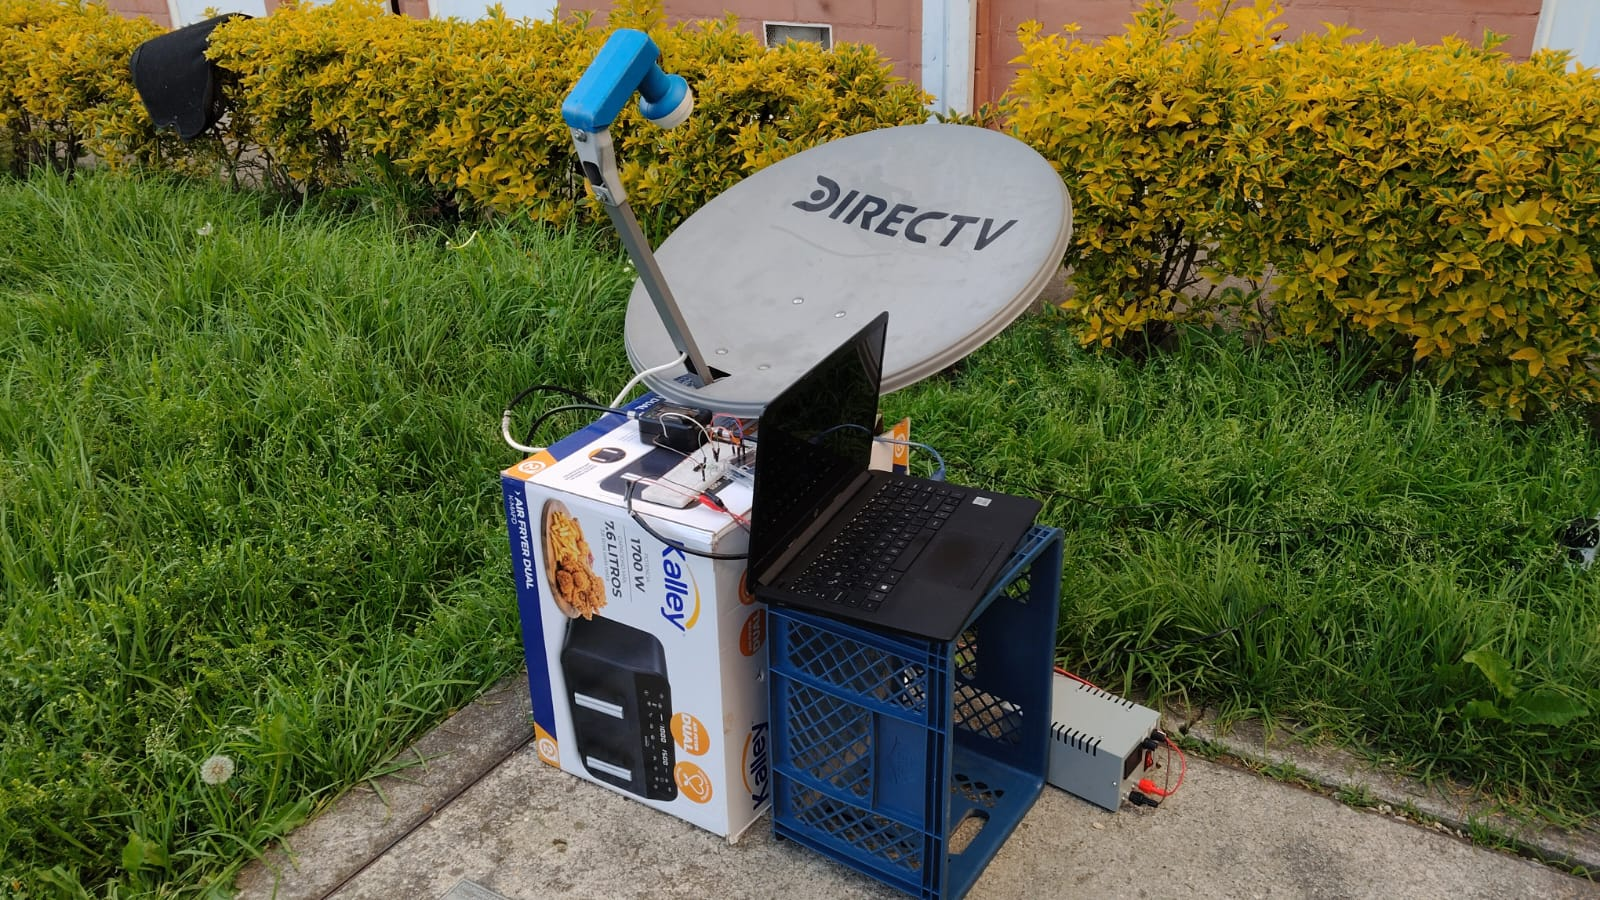
\includegraphics[width=\linewidth]{./Figures/radiotelescope.jpeg}
    \newline
    \small{\textit{Radiotelescopio didáctico de bajo costo}}
  \end{columns}
\end{frame}
